\documentclass{mylib/reporteConCalif}
\graphicspath{ {img/labdisp_pract6/} }

\title{Reporte}
\author{rodrigofranciscopablo }

\subject{Laboratorio de Dispositivos y circuitos electrónicos}
\mytitle{Reporte de práctica 6}
\mysubTitle{Circuitos con diodo Zener}
\students{Francisco Pablo \textsc{Rodrigo}}
\teacher{M.I. Guevara Rodríguez \textsc{Ma. del Socorro}}
\group{8}
\deliverDate{3 de abril de 2019}
\usepackage{mathtools}
\usepackage{amsmath}
\usepackage{float}
\usepackage{tabu}
\usepackage{subfig}

\begin{document}

\coverPage

%\tableofcontents
%\newpage

\section{Objetivos}

\subsection{General}

Analizar y diseñar circuitos electrónicos que contienen diodos semiconductores.

\subsection{Particular}

Analizar, diseñar, simular e implementar circuitos reguladores con diodo Zener.

\section{Introducción}

El diodo zener se puede utilizar para regular una fuente de voltaje. Este semiconductor se fabrica en una amplia variedad de voltajes y potencias.
Estos van desde menos de 2 voltios hasta varios cientos de voltios, y la potencia que pueden disipar va desde 0.25 watts hasta 50 watts o más.
La potencia que disipa un diodo zener es simplemente la multiplicación del voltaje para el que fue fabricado por la corriente que circula por él. Esto es

$$ P_z = V_z \cdot I_z$$

El cálculo del resistor $R_s$ está determinado por la corriente que pedirá la carga (lo que vamos a conectar a esta fuente de voltaje).

Este resistor se puede calcular con la siguiente fórmula

$$R_s = \frac{V_{in min}- V_z}{1.1 \cdot I_{L max}}$$

En donde:
\begin{itemize}
	\item $V_{in min}$ es el valor mínimo del voltaje de entrada.
	\item $I_{L max}$ es el valor de la máxima corriente que pedirá la carga.
\end{itemize}

Una vez conocido Rs, se obtiene la potencia máxima del diodo zener, con ayuda de la siguiente fórmula.

$$P_D = \frac{V_{in min}- V_z}{R_S - I_{L min}} \cdot V_z$$

\newpage
\section{Previo}

\begin{center}
    \begin{tabular}{ | p{4cm} | p{4.5cm} |p{4.5cm} |}
    \hline
    \multicolumn{3}{|c|}{Voltajes y corrientes del diodo Zener} \\
  	\hline

	 & $V_{in}$ mínimo (13 V) & $V_{in}$ máximo (20 V) \\ \hline

	$I_L$ mínima (1mA) & \begin{flalign*} V_Z =  \\ I_Z = \end{flalign*} & \begin{flalign*} V_Z =  \\ I_Z = \end{flalign*} \\ \hline

	$I_L$ máxima (10mA) & \begin{flalign*} V_Z =  \\ I_Z = \end{flalign*} & \begin{flalign*} V_Z =  \\ I_Z = \end{flalign*}\\ \hline

    \end{tabular}
\end{center}

\insertImage{img/labdisp_pract6/one}{Circuito con un $V_{in} = 13 V$ y $I_L = 1 mA$}{8}

\insertImage{img/labdisp_pract6/two}{Circuito con un $V_{in} = 20 V$ y $I_L = 1 mA$}{7}

\insertImage{img/labdisp_pract6/three}{Circuito con un $V_{in} = 13 V$ y $I_L = 10 mA$}{7}

\insertImage{img/labdisp_pract6/four}{Circuito con un $V_{in} = 20 V$ y $I_L = 10 mA$}{7}

\newpage
\section{Desarrollo}

\subsection{Experimento 1}

Para el experimento 1 en donde la corriente es la mínima (1 mA) y el voltaje es el mínimo (13 V) obtuvimos los siguientes resultados.

\begin{figure}[H]%
    \centering
    \subfloat[$V_z$ = 9.15 V]{{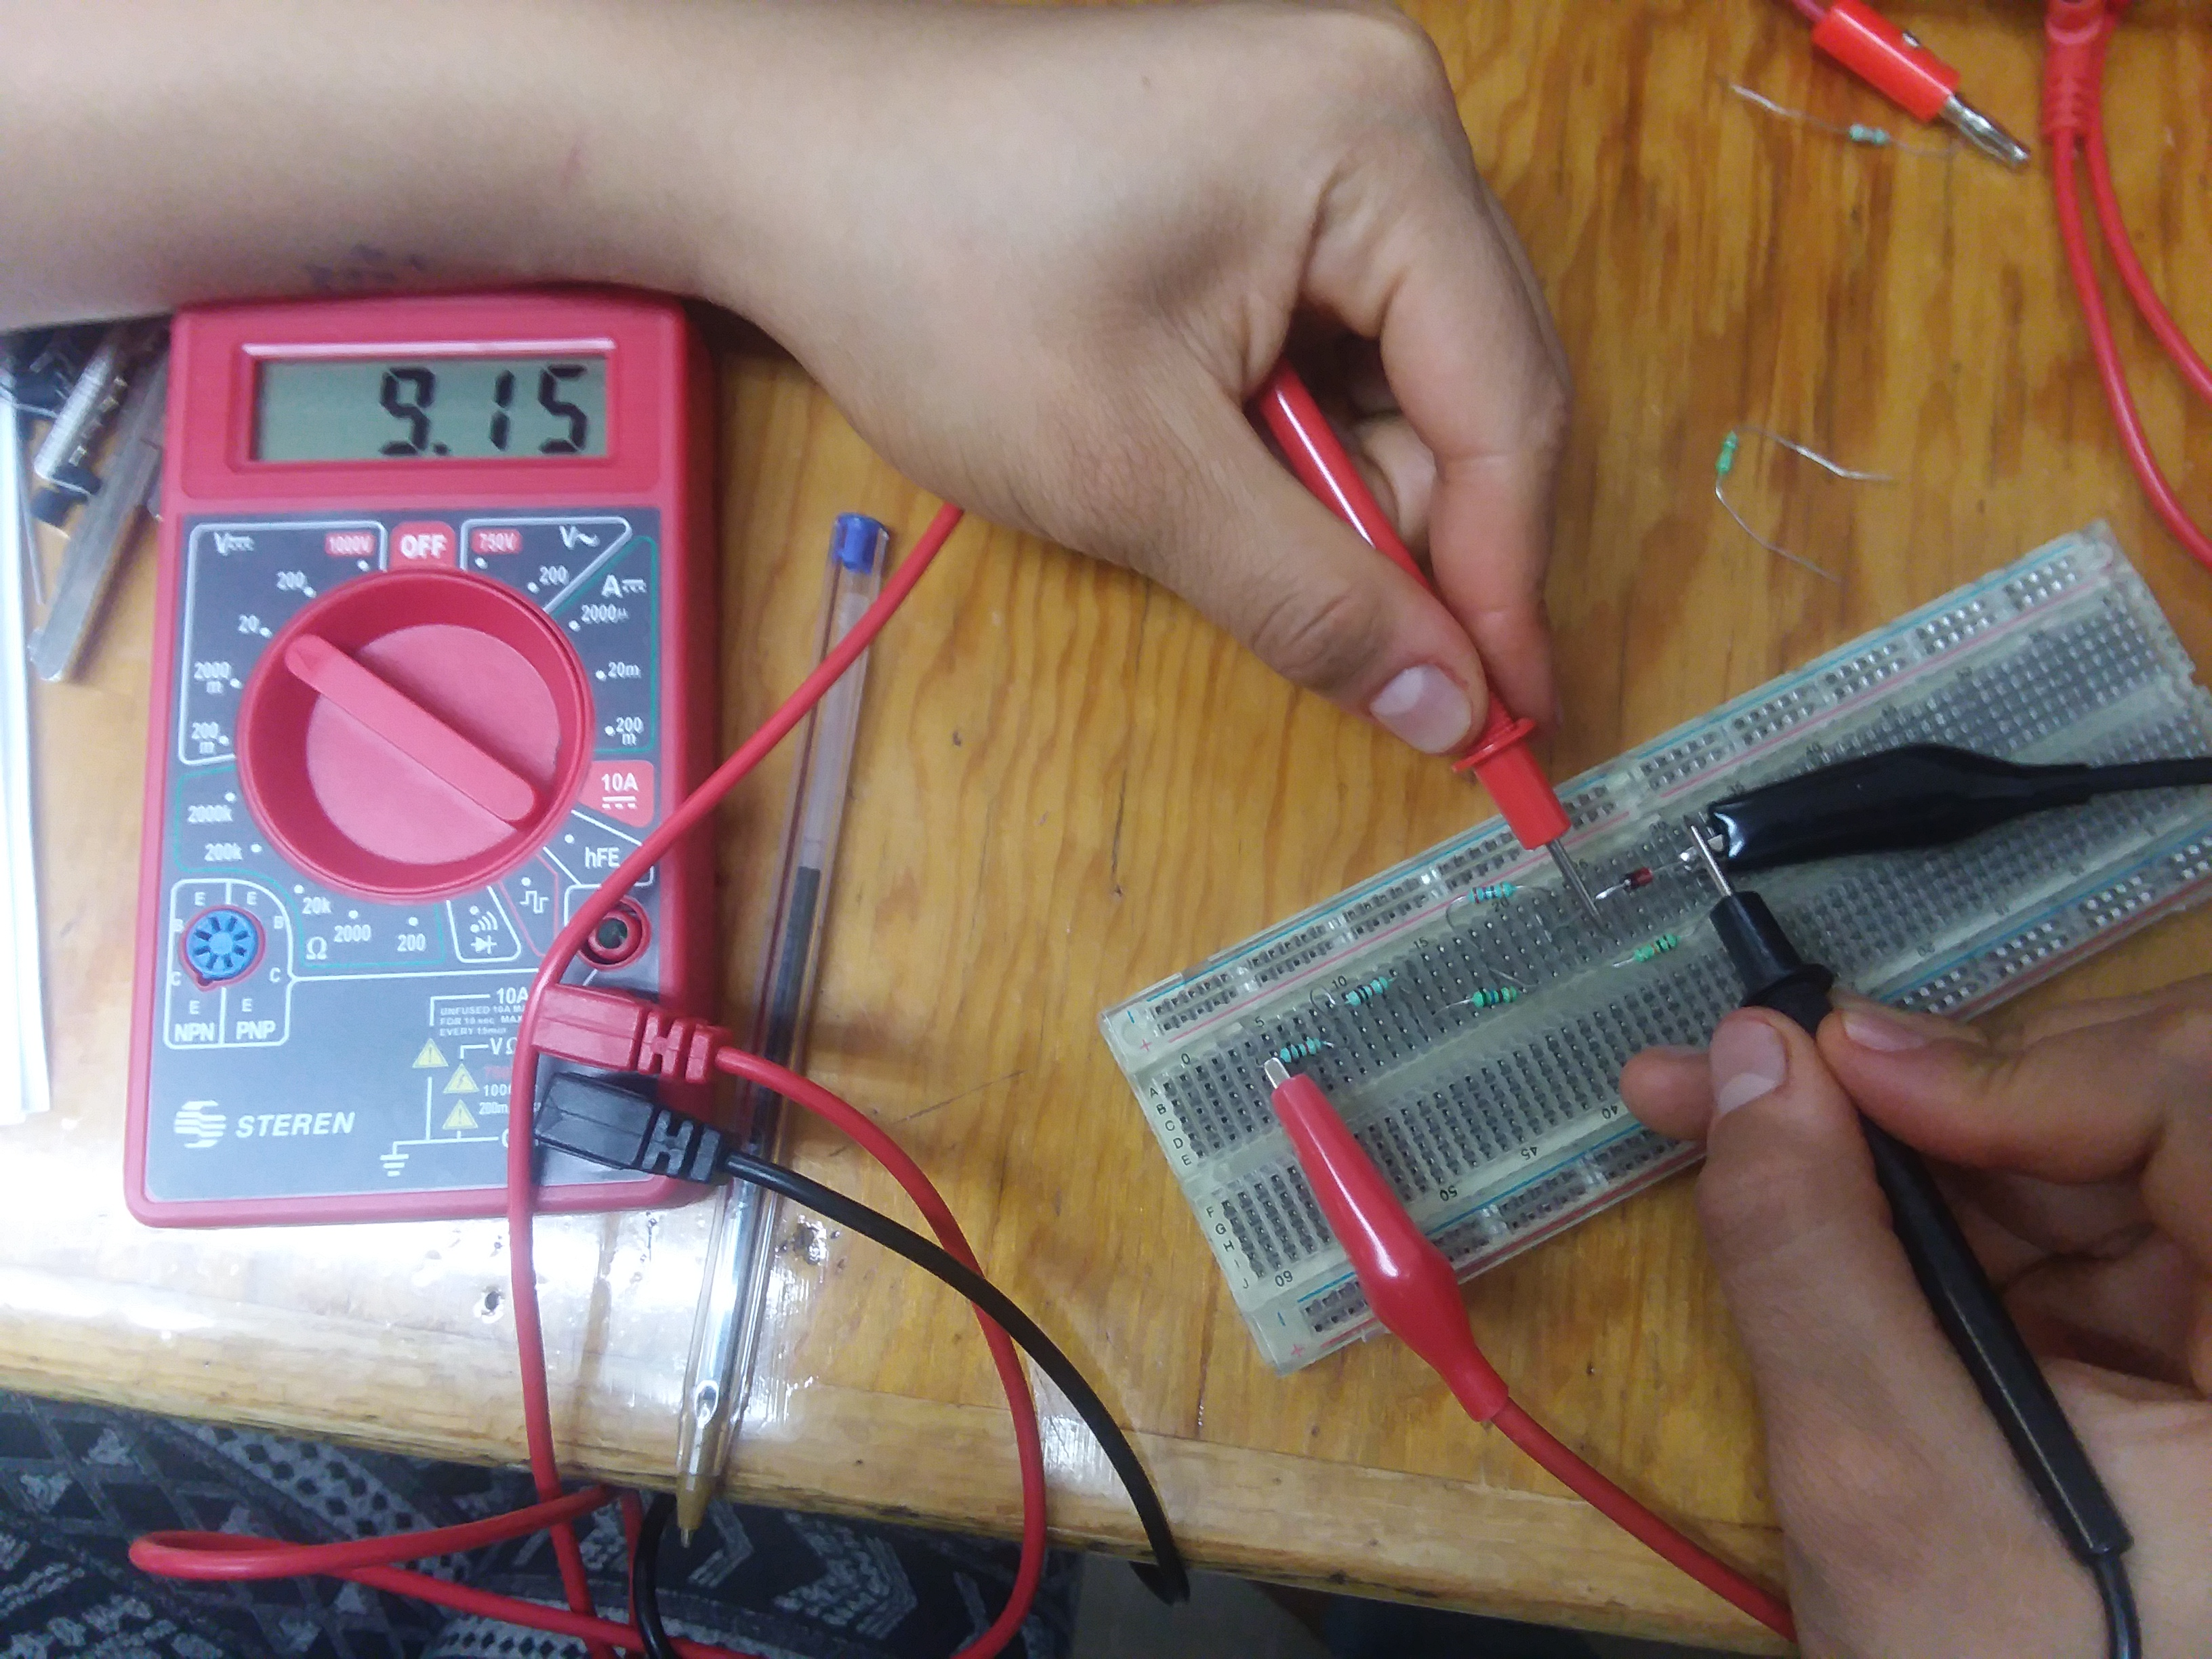
\includegraphics[width=7cm]{image8} }}%
    \qquad
    \subfloat[I = 1.19 mA]{{
\includegraphics[width=7cm]{image3} }}%
    \caption{Voltaje y corriente del diodo Zener}%
    \label{fig:example}%
\end{figure}

\subsection{Experimento 2}

Para el experimento 2 en donde la corriente es la mínima (1 mA) y el voltaje es el máximo (20 V) obtuvimos los siguientes resultados.

\begin{figure}[H]%
    \centering
    \subfloat[$V_z$ = 7.44 V]{{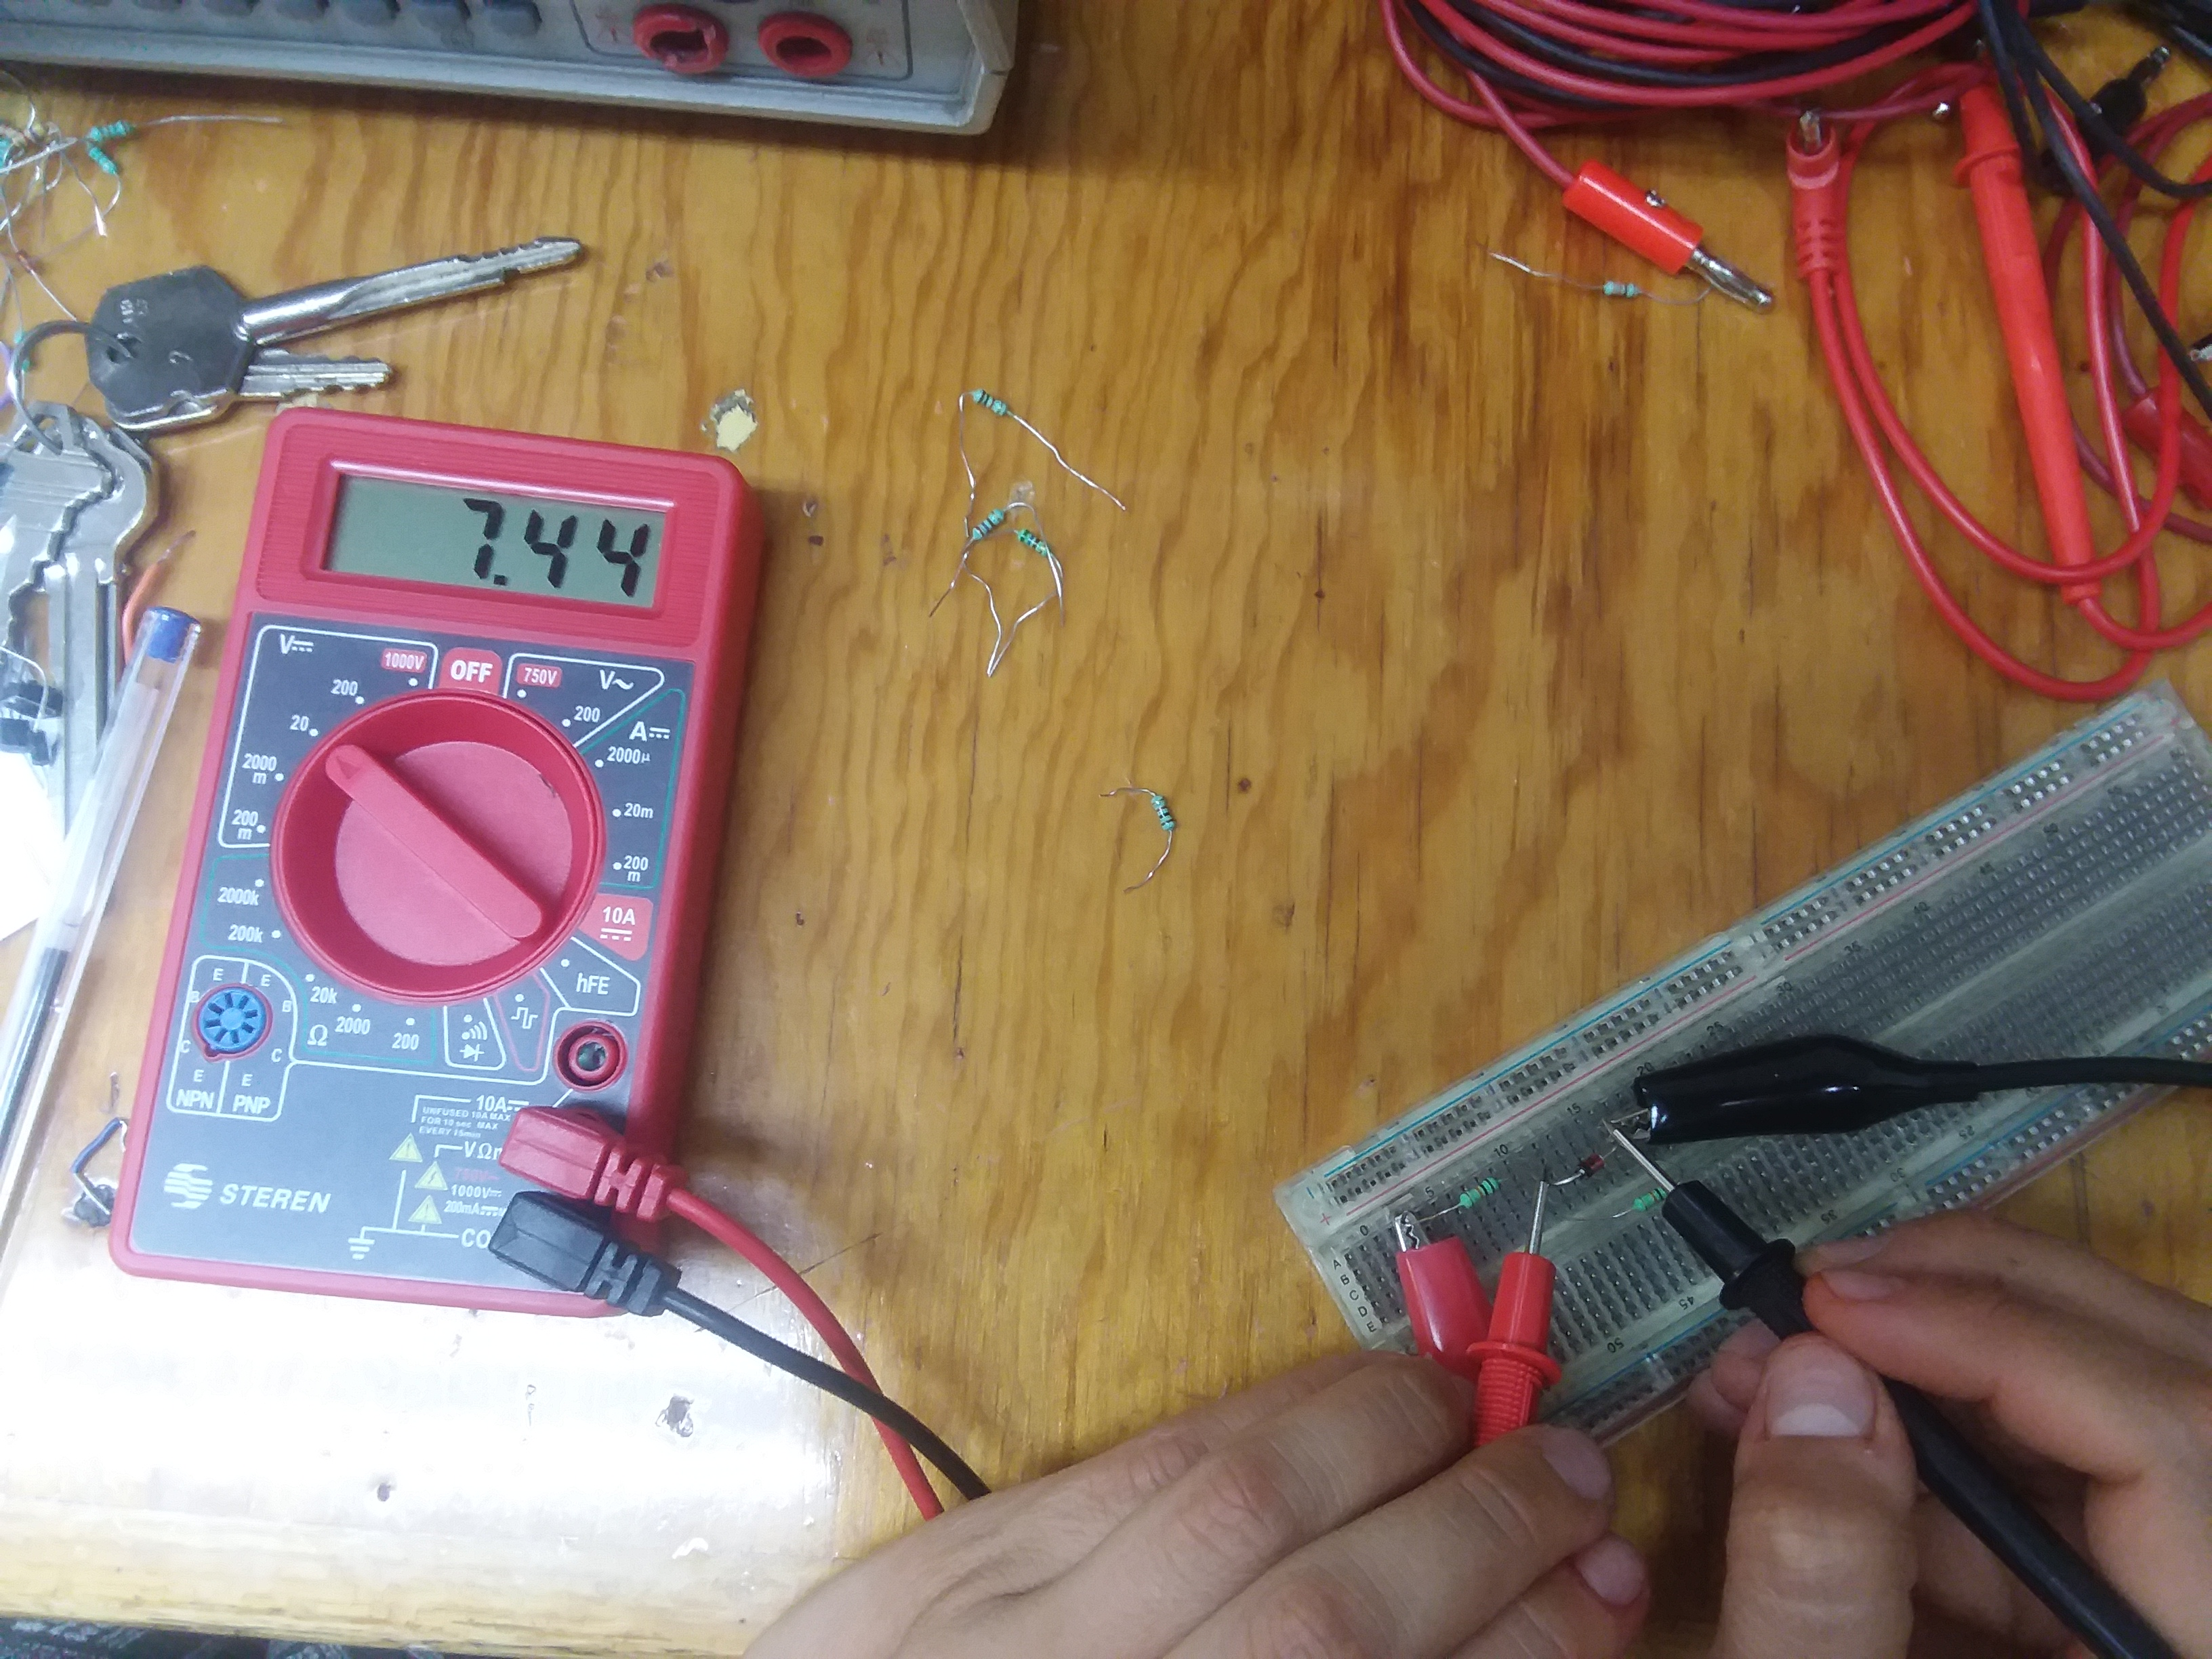
\includegraphics[width=7cm]{image4} }}%
    \qquad
    \subfloat[I = 1.19 mA]{{
\includegraphics[width=7cm]{image3} }}%
    \caption{Voltaje y corriente del diodo Zener}%
    \label{fig:example}%
\end{figure}

\subsection{Experimento 3}

Para el experimento 3 en donde la corriente es la máxima(10 mA) y el voltaje es el mínimo (13 V) obtuvimos los siguientes resultados.

\begin{figure}[H]%
    \centering
    \subfloat[$V_z$ = 10.34 V]{{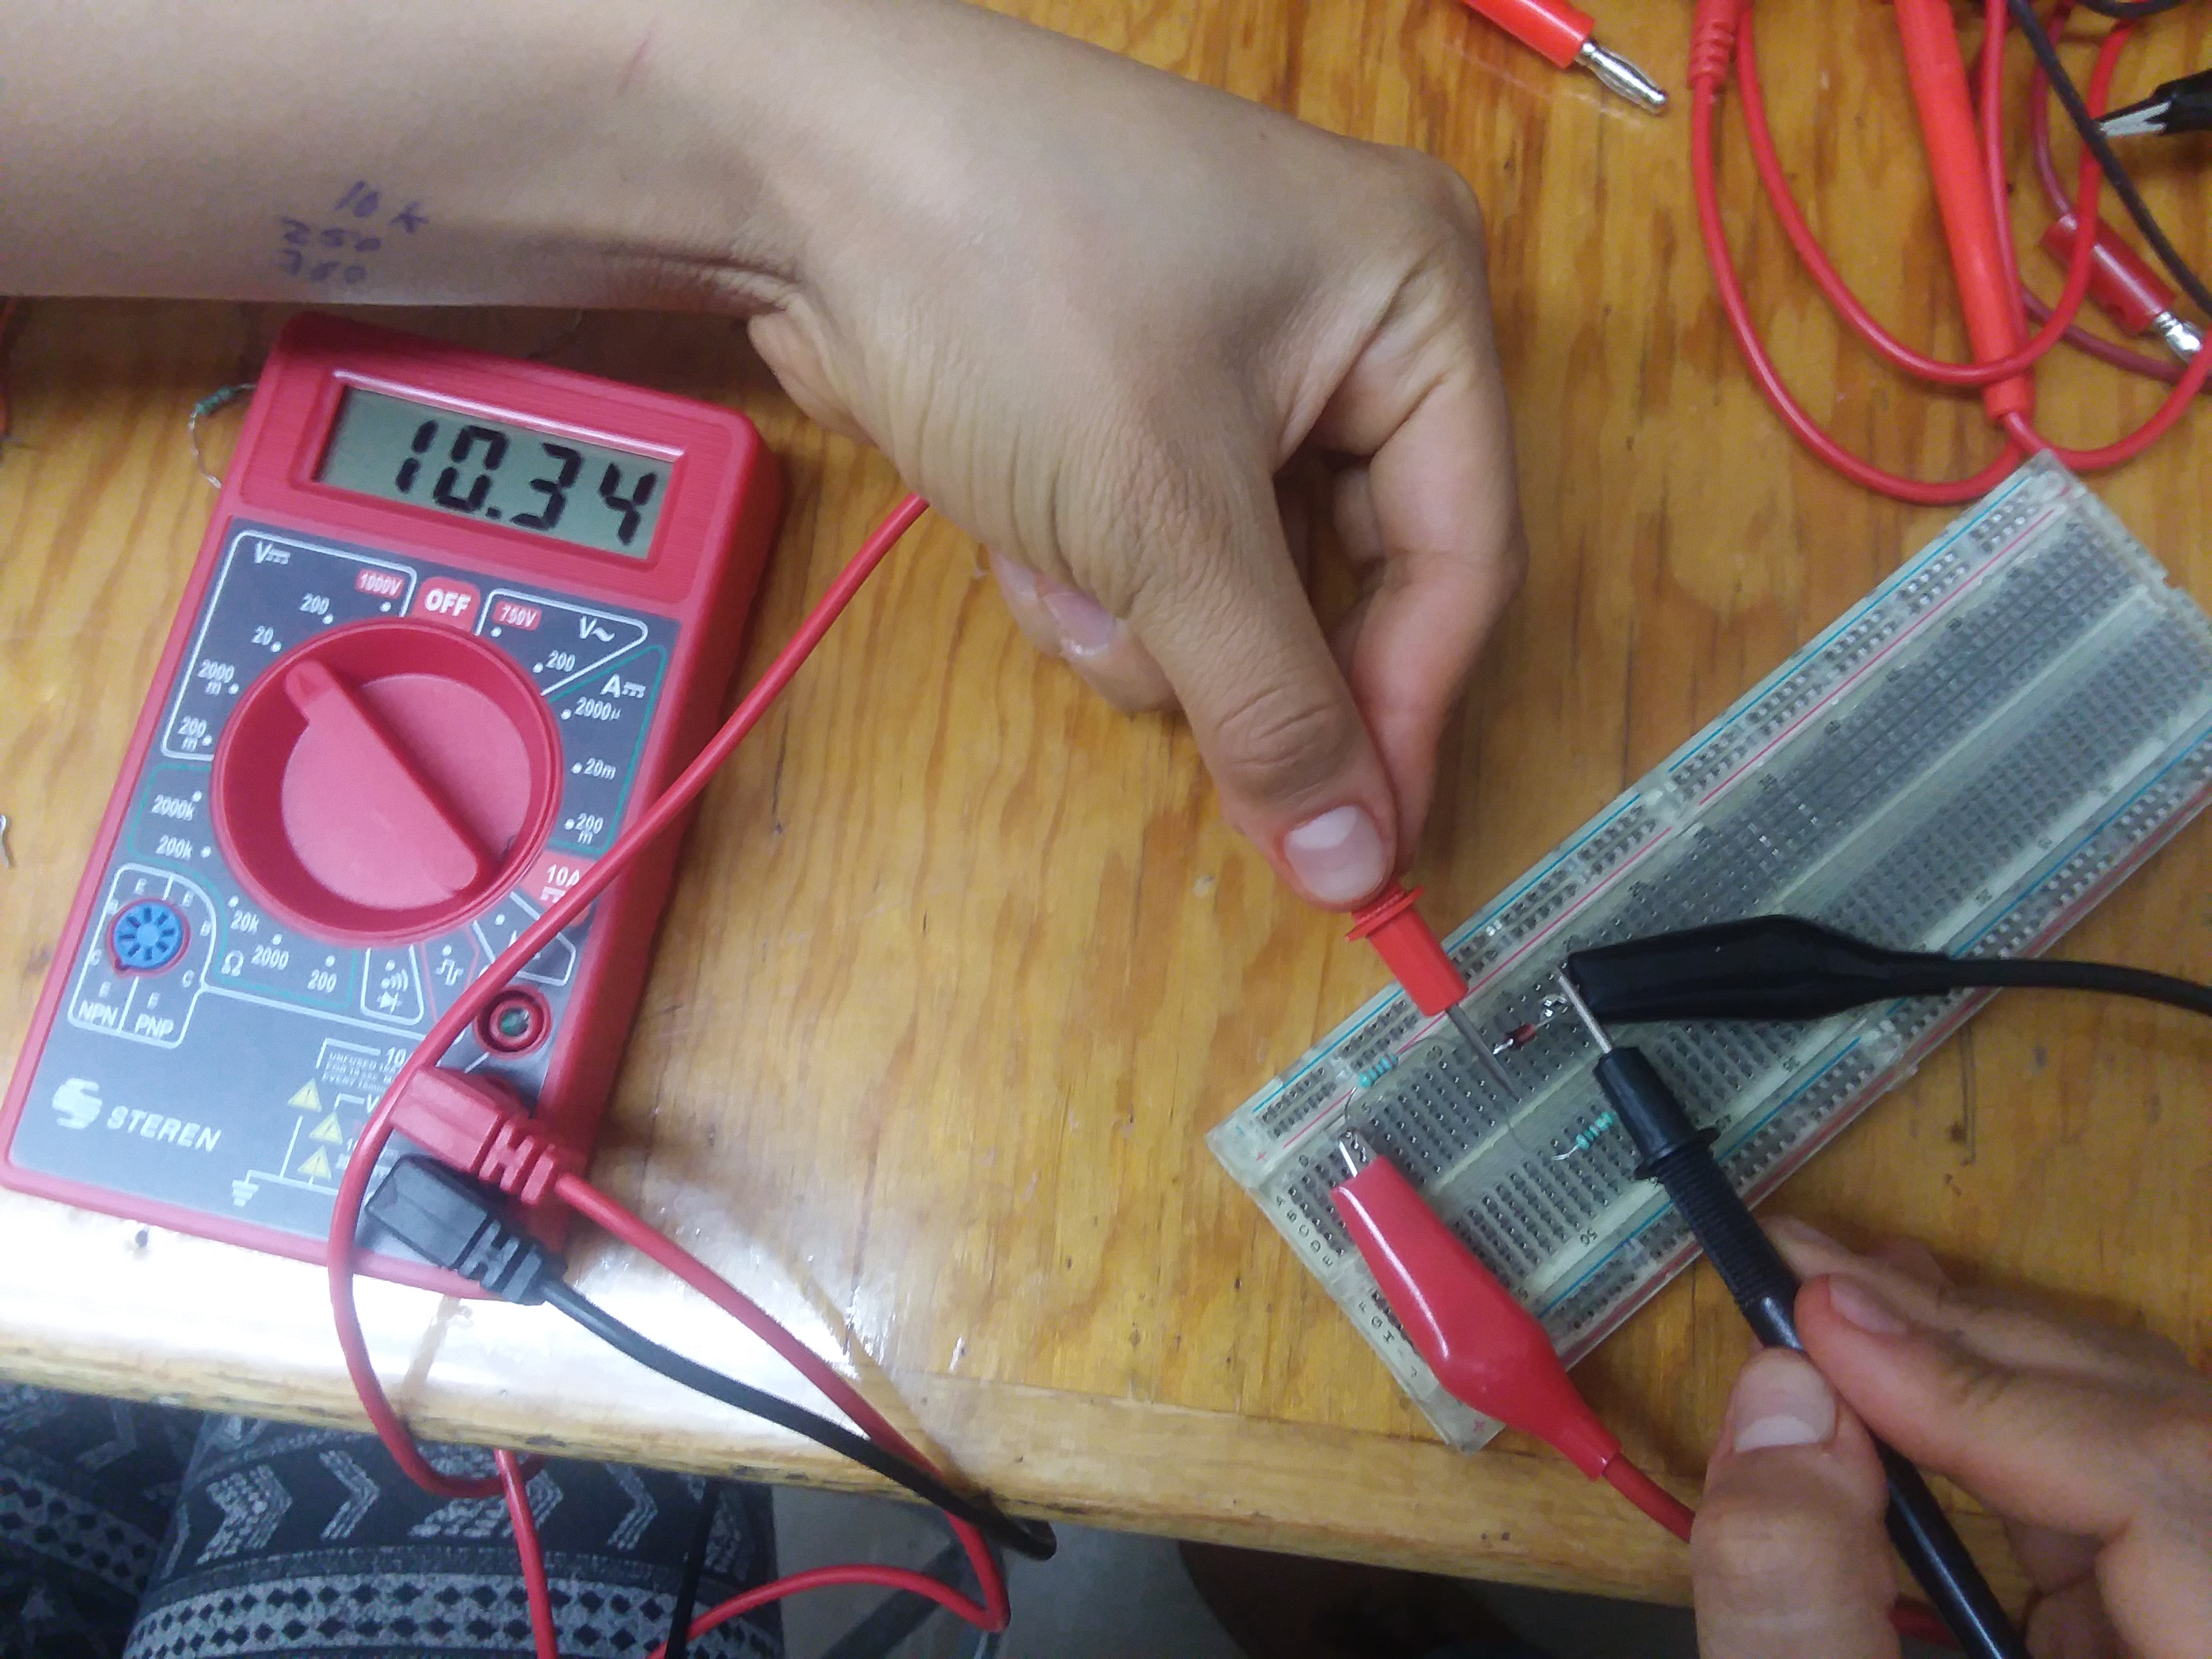
\includegraphics[width=7cm]{image2} }}%
    \qquad
    \subfloat[I = 36.3 mA]{{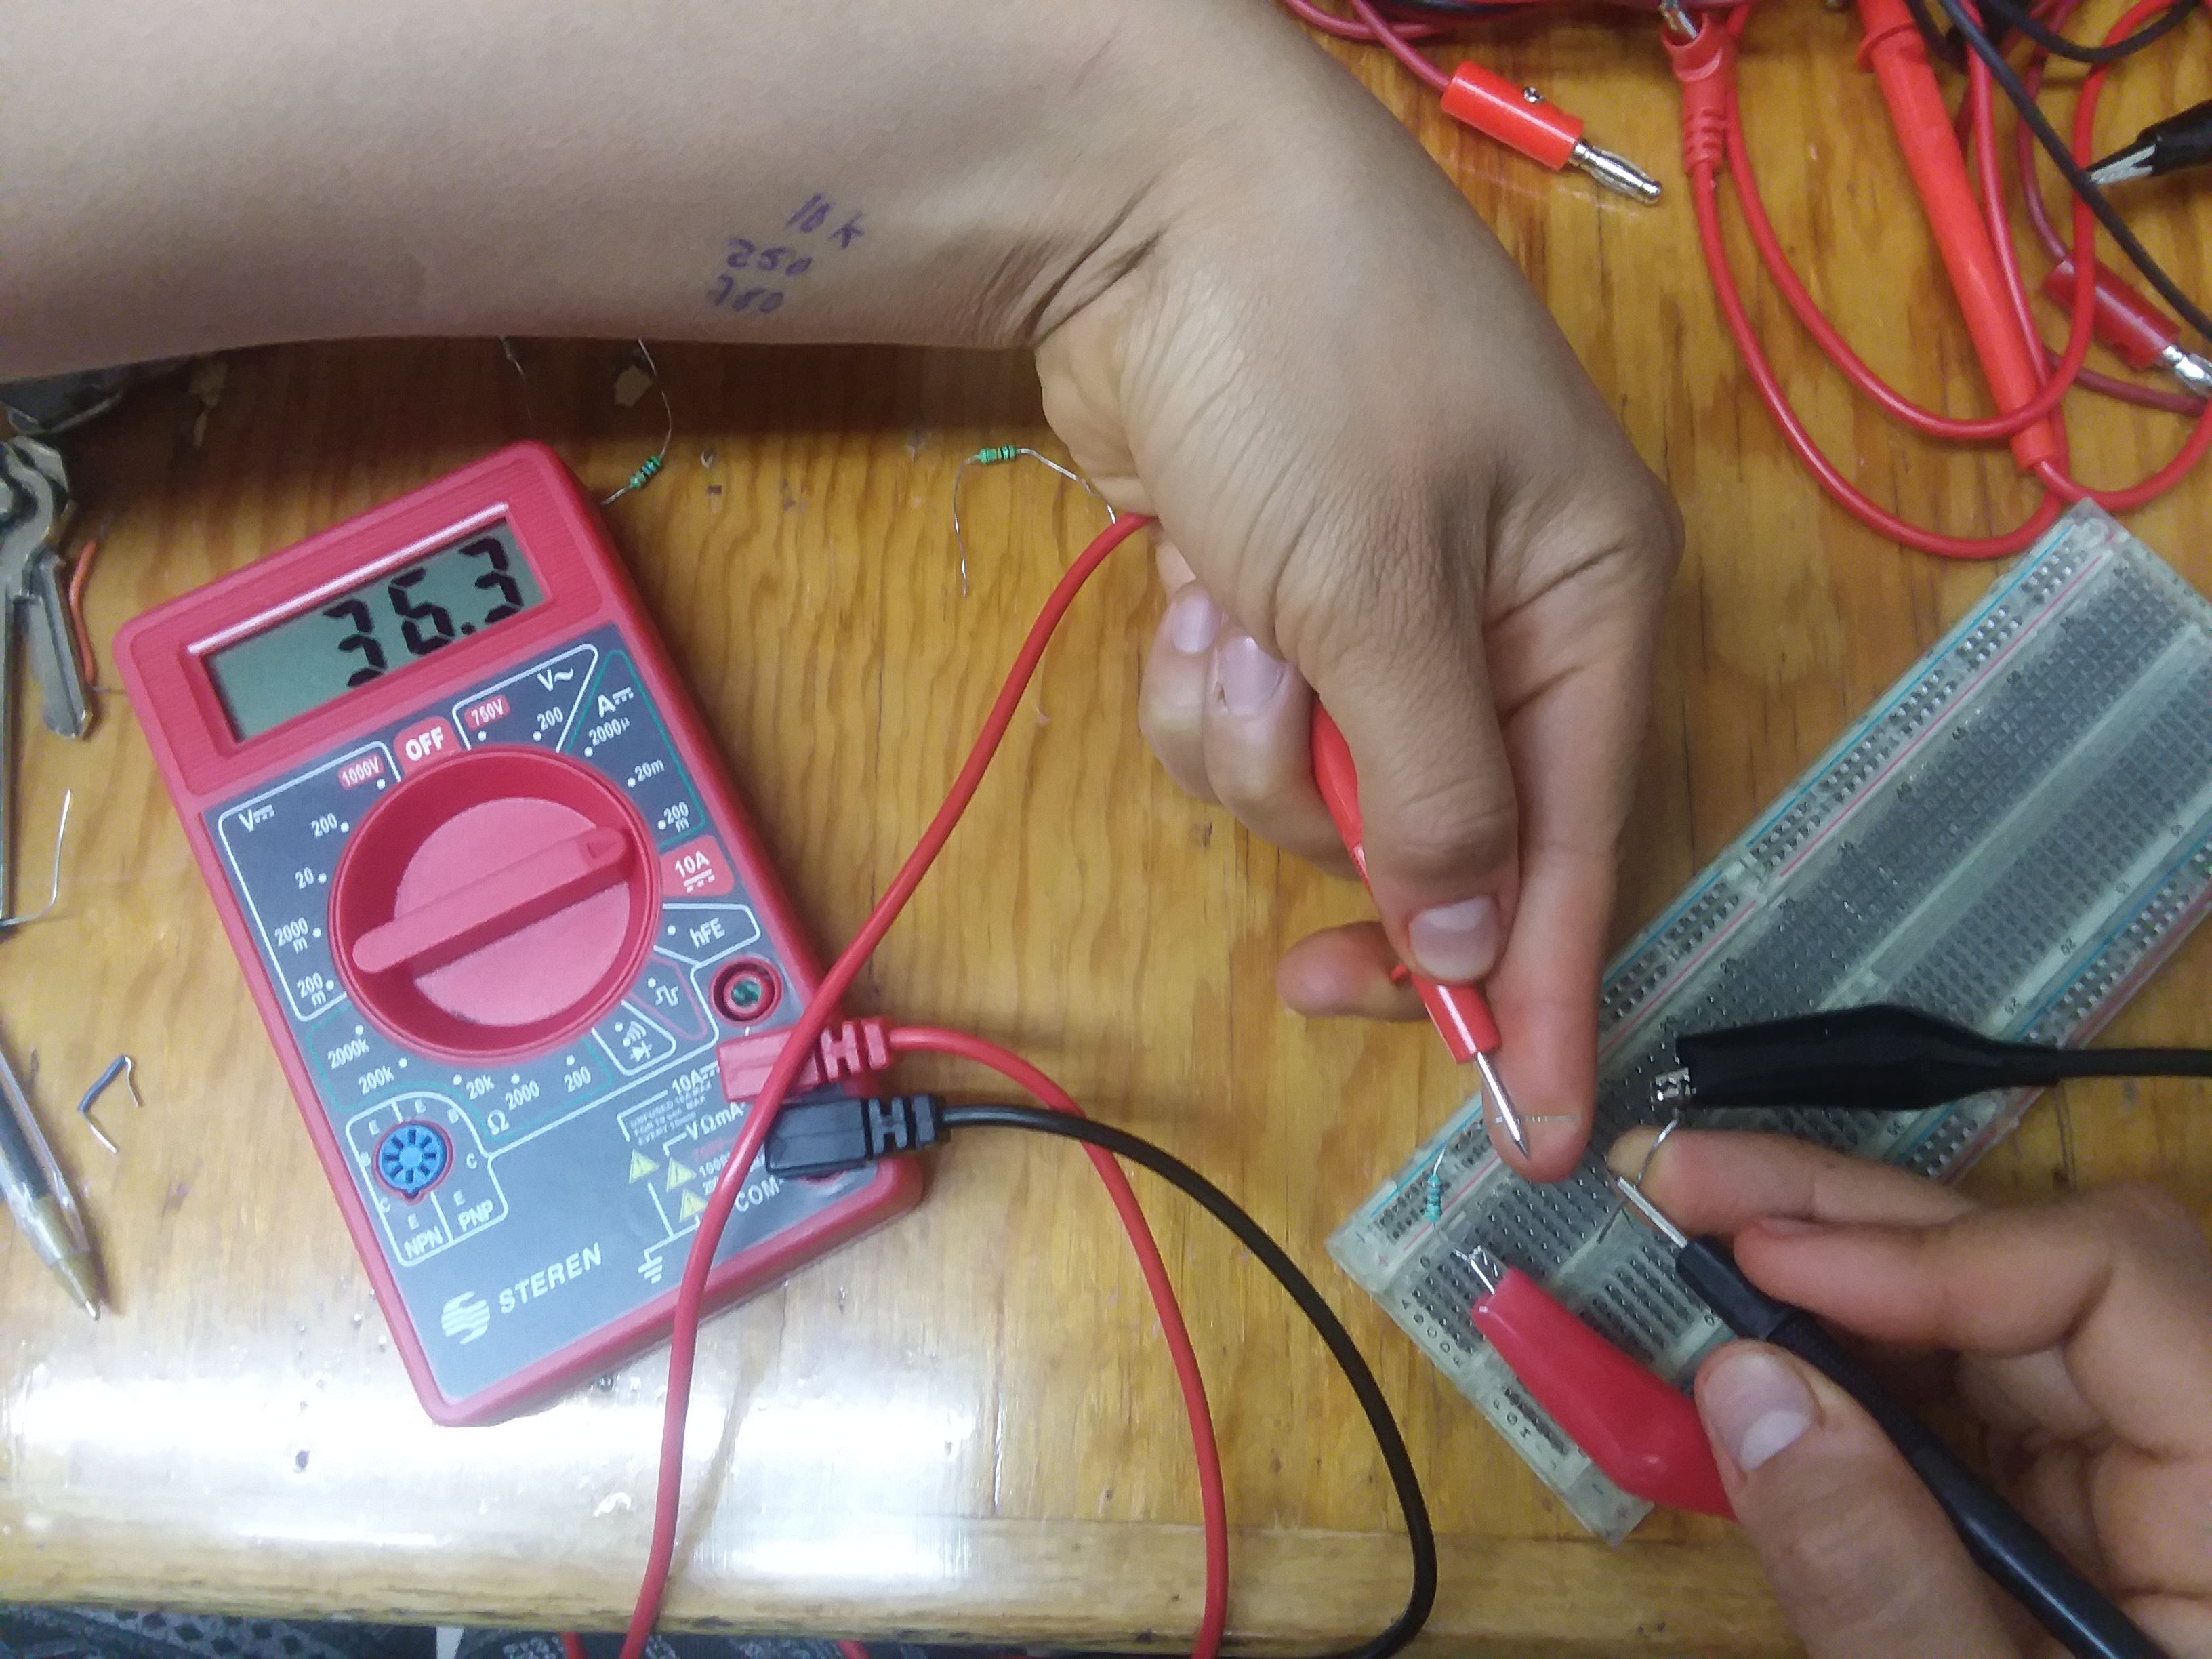
\includegraphics[width=7cm]{image1} }}%
    \caption{Voltaje y corriente del diodo Zener}%
    \label{fig:example}%
\end{figure}

\subsection{Experimento 4}

Para el experimento 4 en donde la corriente es la máxima(10 mA) y el voltaje es el máximo (20 V) obtuvimos los siguientes resultados.

\begin{figure}[H]%
    \centering
    \subfloat[$V_z$ = 10.19 V]{{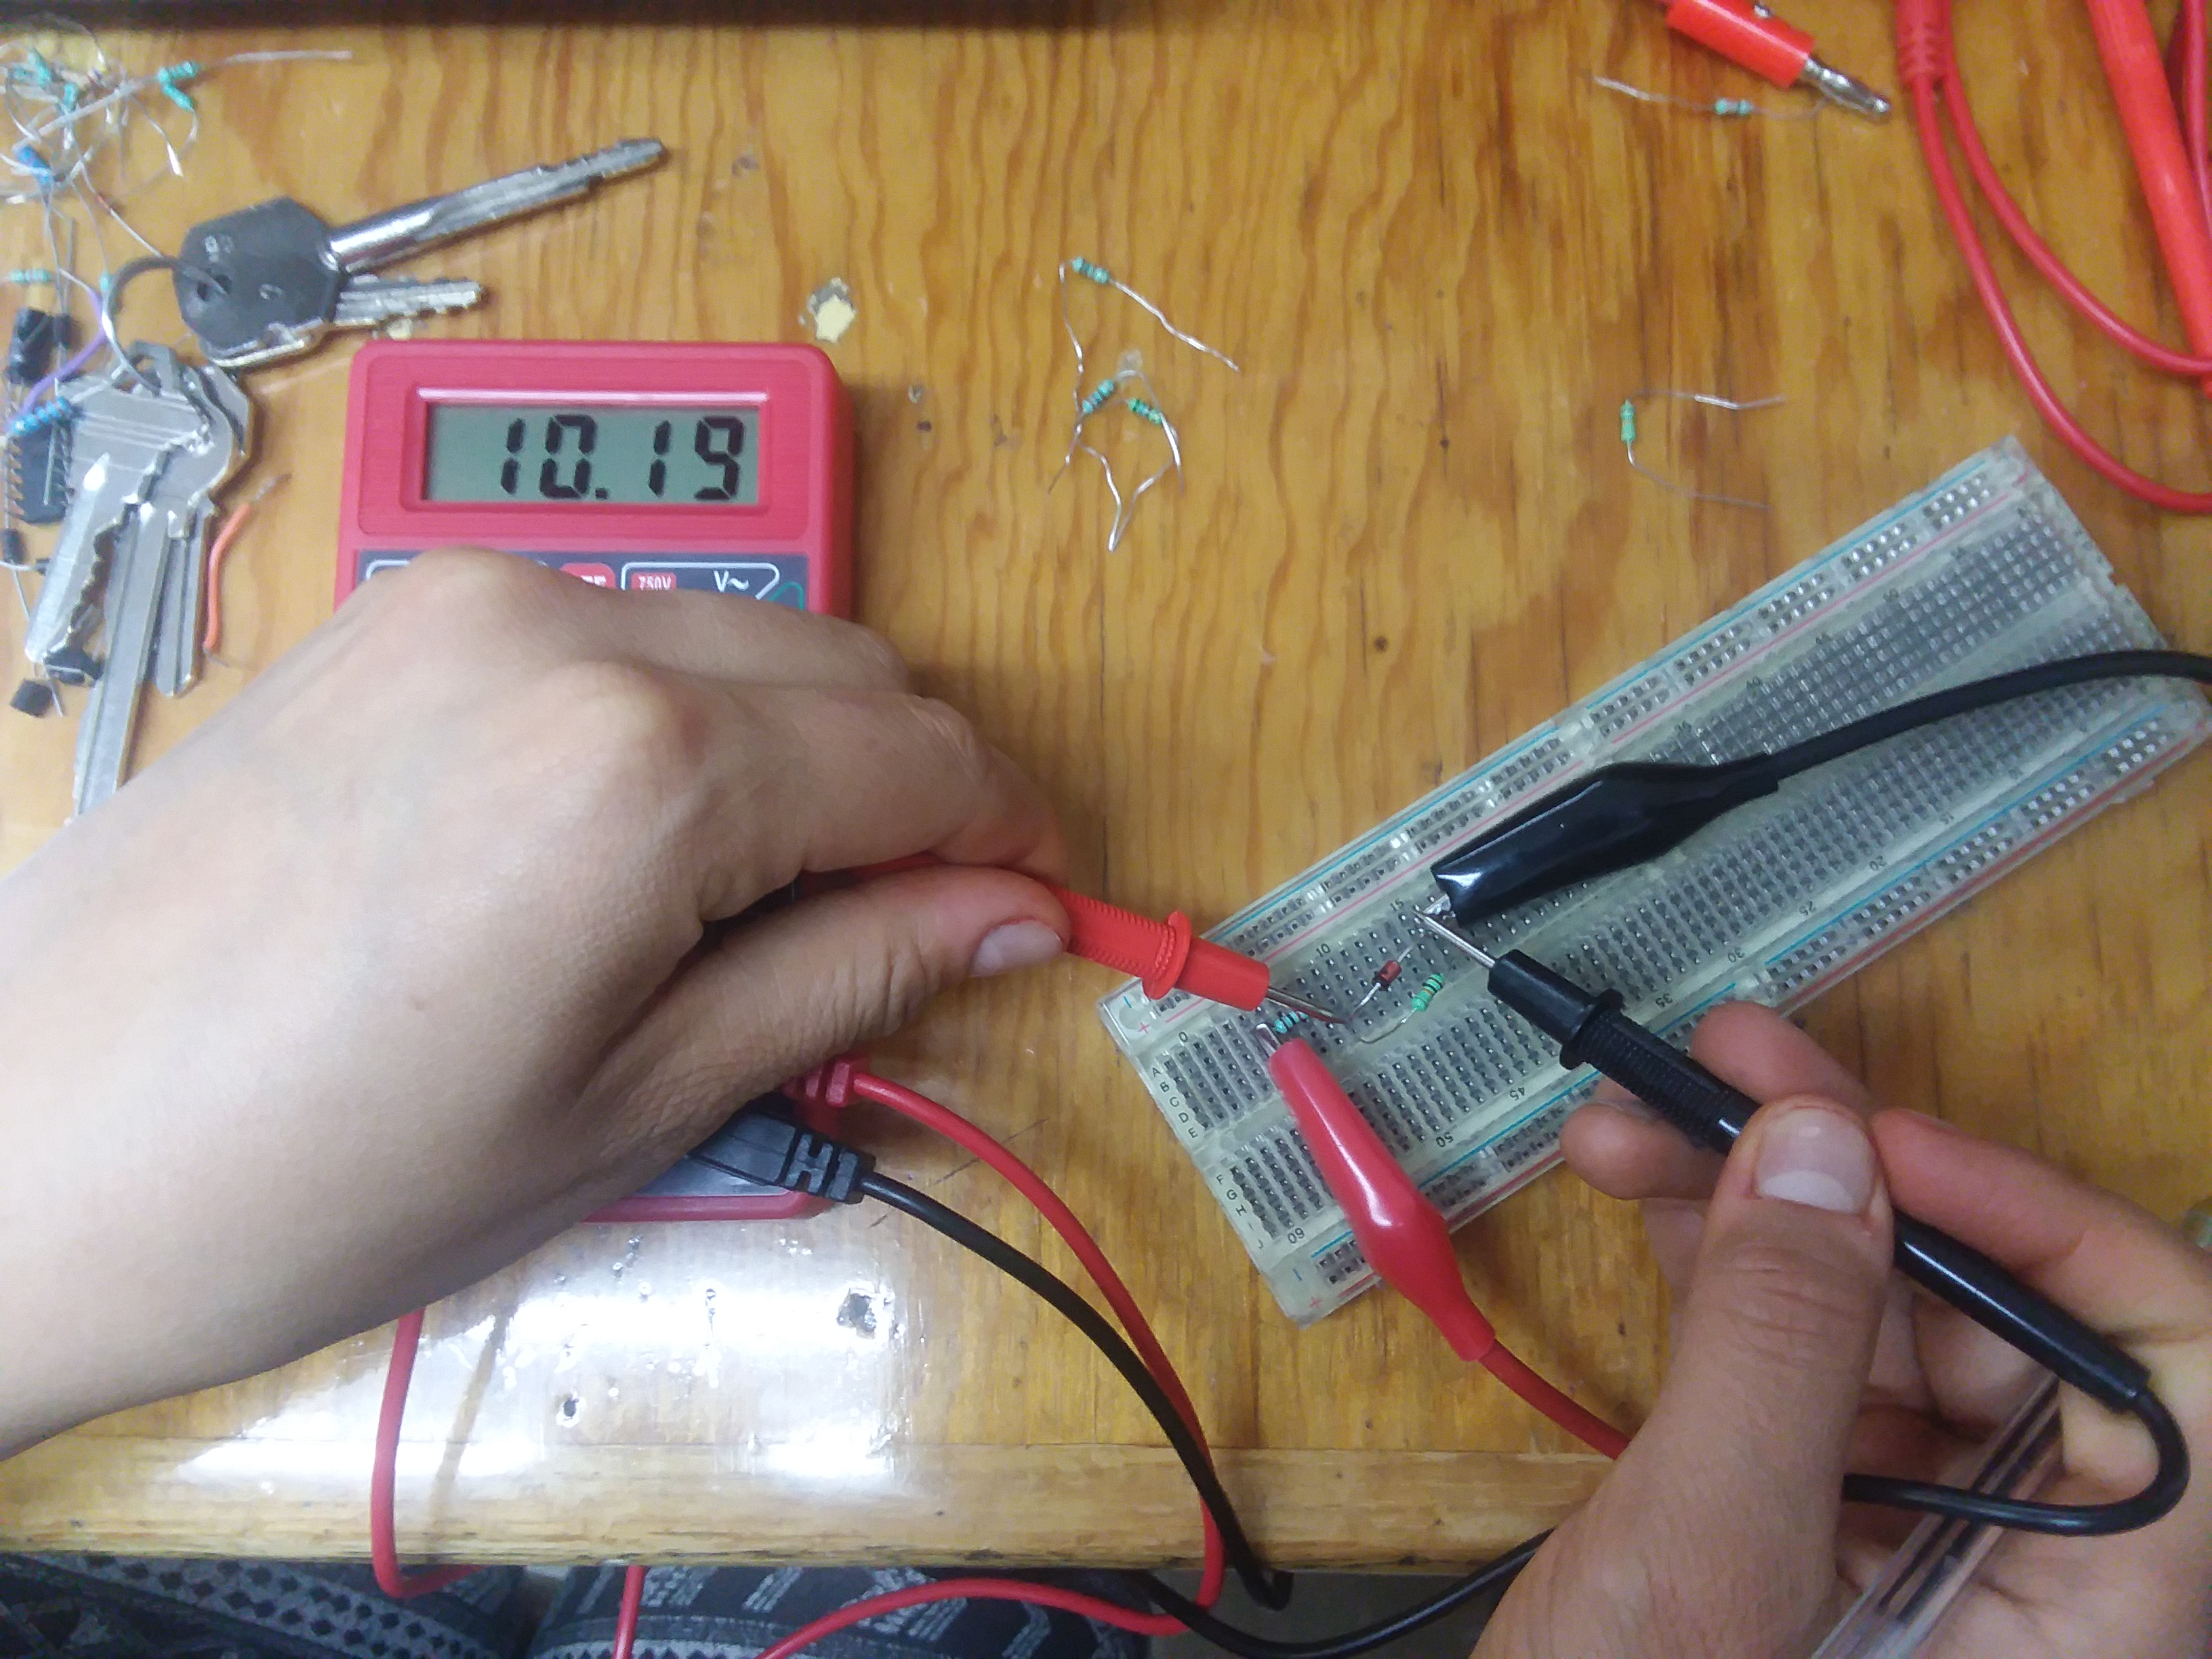
\includegraphics[width=7cm]{image6} }}%
    \qquad
    \subfloat[I = 9.9 mA]{{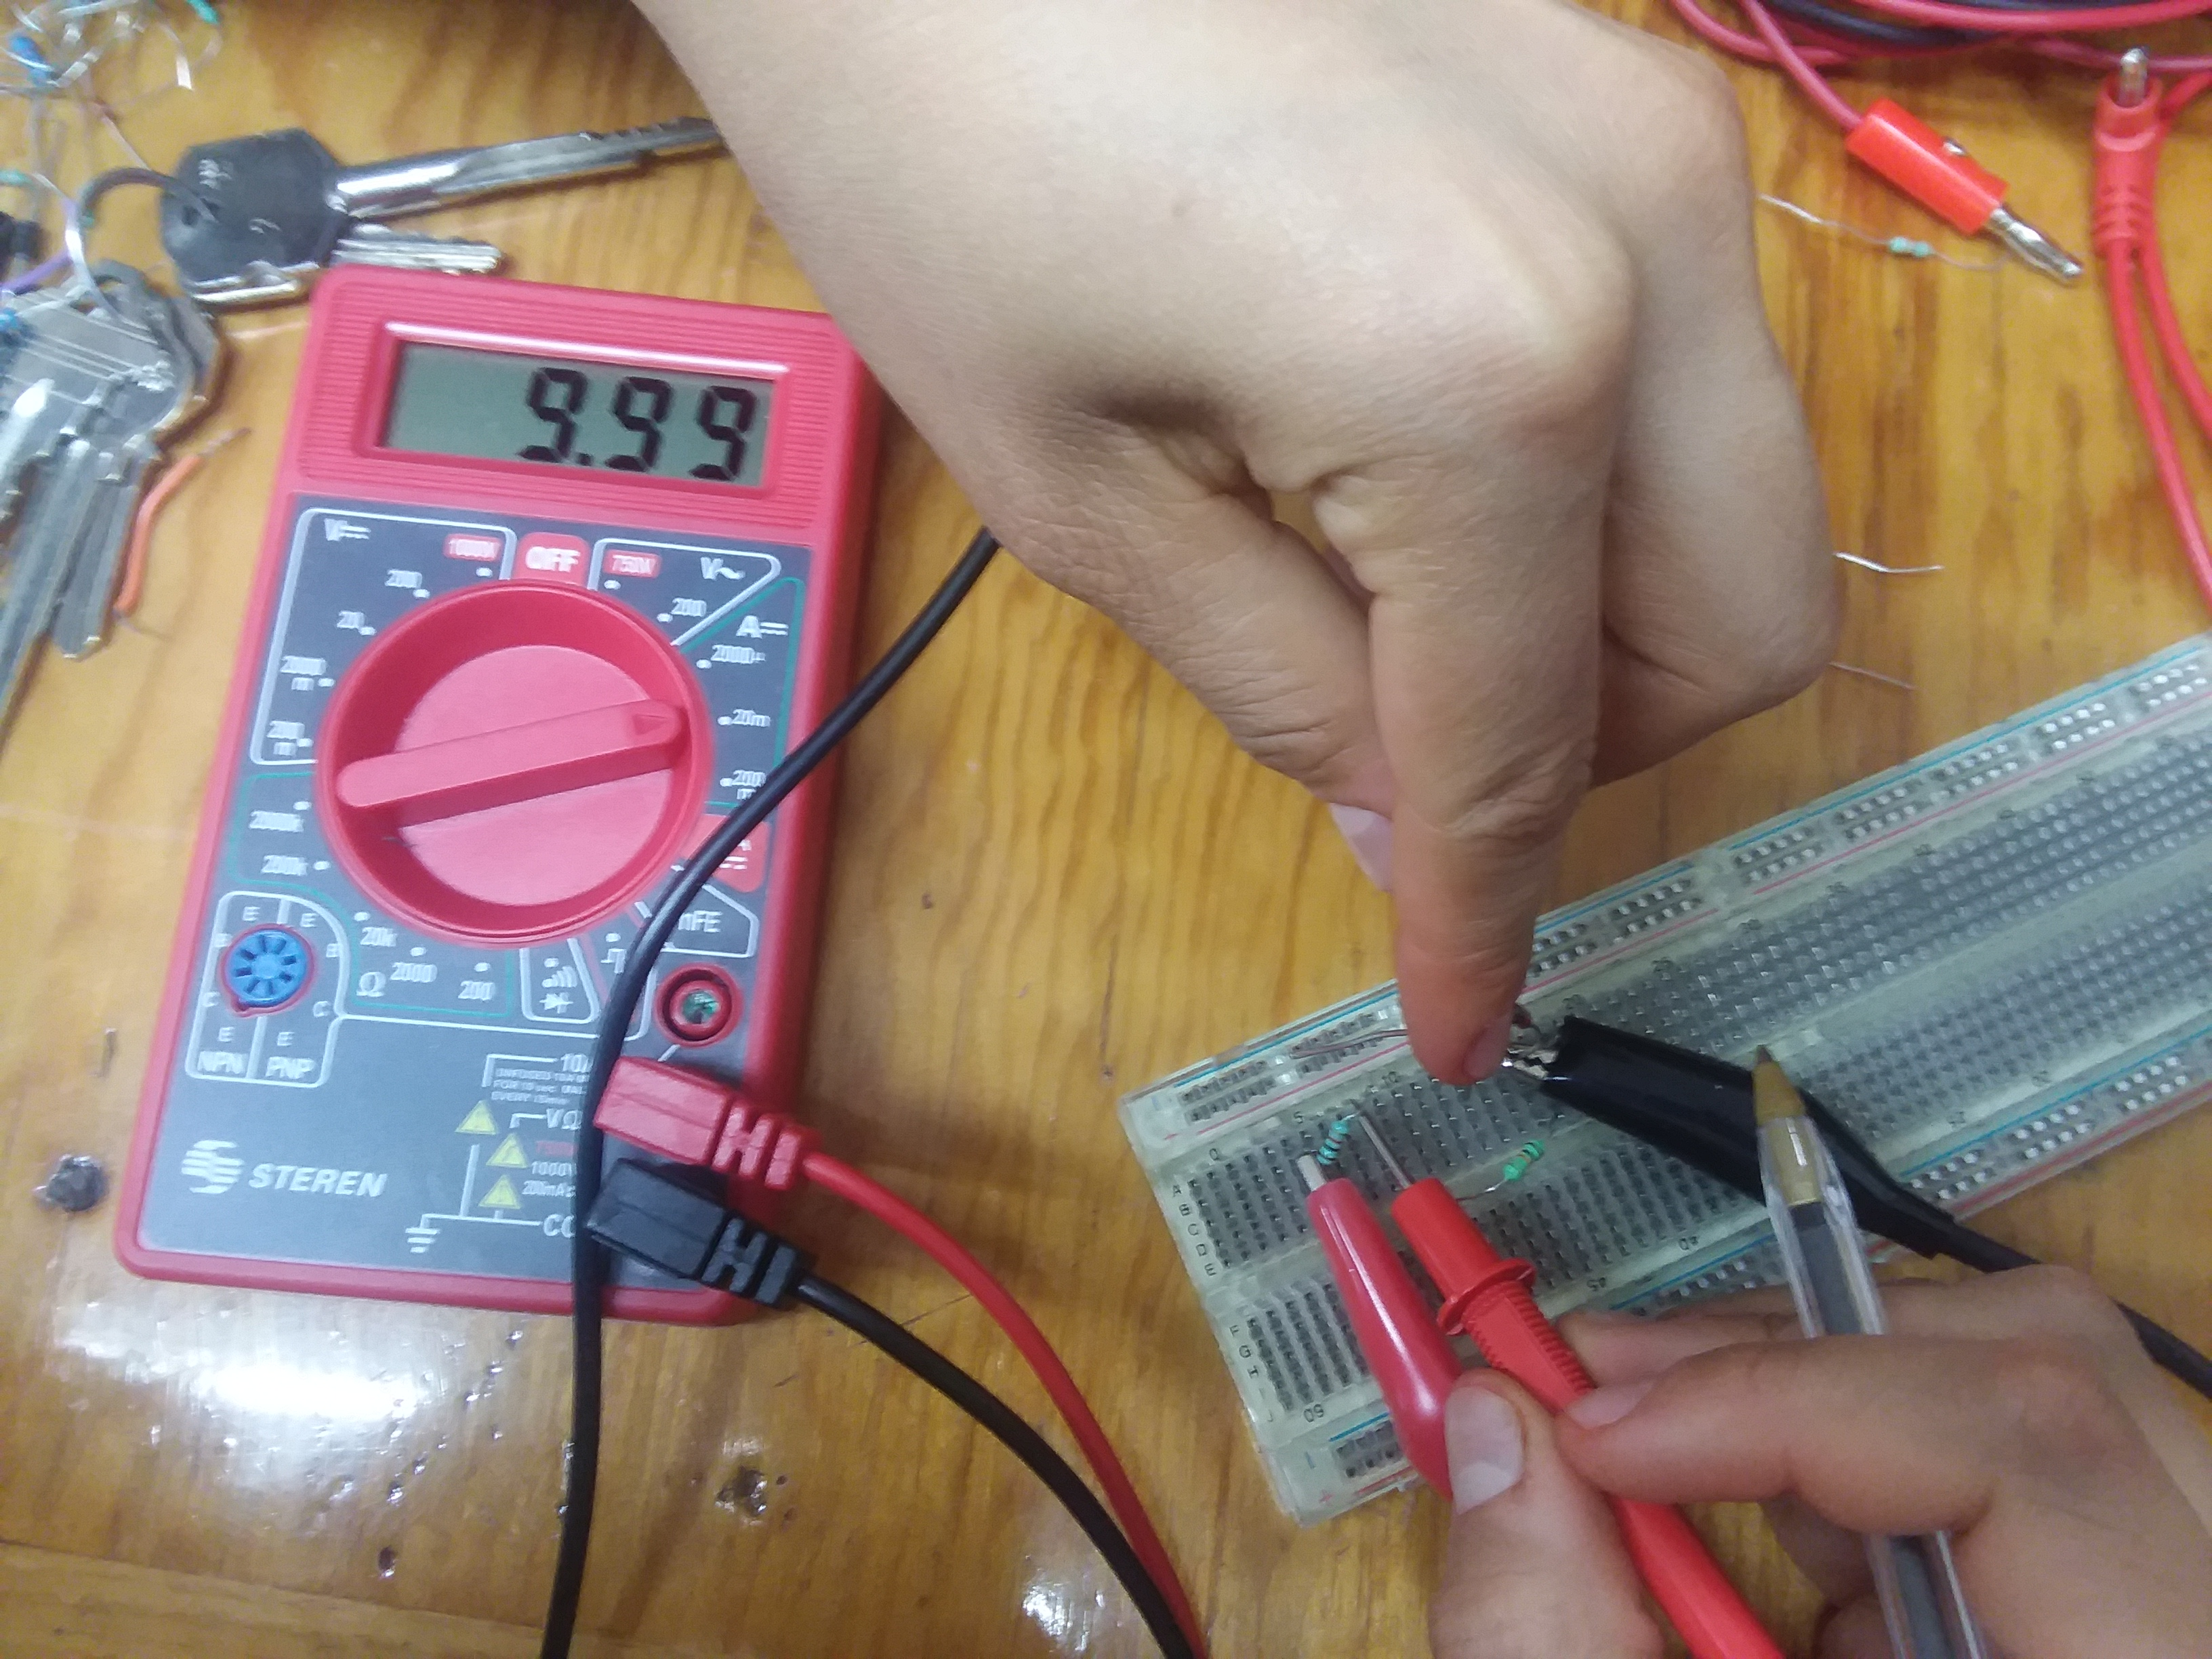
\includegraphics[width=7cm]{image5} }}%
    \caption{Voltaje y corriente del diodo Zener}%
    \label{fig:example}%
\end{figure}

Observamos que al ir variando el voltaje de la fuente, el diodo Zener intentó conservar su valor de voltaje, al no ser un dispositivo tan preciso lo máximo que pudo hacer fue estar en valores entre 7.30 V y 11 V.
Esta forma de regular el voltaje se debe a la curva de polizarización del diodo Zener, la cual se presenta a continuación.

\insertImage{zener}{Curva de un diodo semiconductor. En azúl se representa la región en directa y en rojo la región en inversa.}{10}

\section{Conclusiones}

Observamos el diodo Zener se comporta como un regulador de voltaje. De esta práctica aprendimos que debemos de verificar que el diodo que compremos con ciertos valores nominales sean verdaderos, es decir, si nos venden un diodo de 10 V a 1 watt es importante que verificar que efectivamente el diodo regule 10 volts y no menos ya que si regula menos podríamos dañar los componentes que este protegiendo.

Básicamente, se estructura igual que un diodo semiconductor o diodo de pequeña señal. La gran diferencia, es que el diodo zener trabaja en la región de ruptura o Zener. Esta región se da cuando el diodo se polariza en inversa. Por lo tanto, el diodo Zener, se utilizará como un diodo polarizado en inversa y gracias a esto es que podemos usarlo como regulador de voltaje.

\end{document}
